%%%%%%%%%%%%%%%%%%%%%%%%%%%%%%%%%%%%%%%%%%%%%%%%%%%%%%%%%%%%%%%%%%%%%%%%%%%%%
%% Original default rstudio/pandoc latex file
%% upated by @jhollist 09/15/2014
%% inspired by @cboetting https://github.com/cboettig/template and
%% @rmflight blog posts:
%% http://rmflight.github.io/posts/2014/07/analyses_as_packages.html 
%% http://rmflight.github.io/posts/2014/07/vignetteAnalysis.html).  
%%%%%%%%%%%%%%%%%%%%%%%%%%%%%%%%%%%%%%%%%%%%%%%%%%%%%%%%%%%%%%%%%%%%%%%%%%%%%

\documentclass[11pt,]{article}
\usepackage[T1]{fontenc}
\usepackage{lmodern}
\usepackage{amssymb,amsmath}
\usepackage{ifxetex,ifluatex}
\usepackage{fixltx2e} % provides \textsubscript
% use upquote if available, for straight quotes in verbatim environments
\IfFileExists{upquote.sty}{\usepackage{upquote}}{}
\ifnum 0\ifxetex 1\fi\ifluatex 1\fi=0 % if pdftex
  \usepackage[utf8]{inputenc}
\else % if luatex or xelatex
  \ifxetex
    \usepackage{mathspec}
    \usepackage{xltxtra,xunicode}
  \else
    \usepackage{fontspec}
  \fi
  \defaultfontfeatures{Mapping=tex-text,Scale=MatchLowercase}
  \newcommand{\euro}{€}
\fi
% use microtype if available
\IfFileExists{microtype.sty}{\usepackage{microtype}}{}
\usepackage{longtable,booktabs}
\usepackage{graphicx}
% Redefine \includegraphics so that, unless explicit options are
% given, the image width will not exceed the width of the page.
% Images get their normal width if they fit onto the page, but
% are scaled down if they would overflow the margins.
\makeatletter
\def\ScaleIfNeeded{%
  \ifdim\Gin@nat@width>\linewidth
    \linewidth
  \else
    \Gin@nat@width
  \fi
}
\makeatother
\let\Oldincludegraphics\includegraphics
{%
 \catcode`\@=11\relax%
 \gdef\includegraphics{\@ifnextchar[{\Oldincludegraphics}{\Oldincludegraphics[width=\ScaleIfNeeded]}}%
}%
\ifxetex
  \usepackage[setpagesize=false, % page size defined by xetex
              unicode=false, % unicode breaks when used with xetex
              xetex]{hyperref}
\else
  \usepackage[unicode=true]{hyperref}
\fi
\hypersetup{breaklinks=true,
            bookmarks=true,
            pdfauthor={},
            pdftitle={Associations between chlorophyll a and various microcystin health advisory Concentrations},
            colorlinks=true,
            citecolor=blue,
            urlcolor=blue,
            linkcolor=magenta,
            pdfborder={0 0 0}}
\urlstyle{same}  % don't use monospace font for urls
\setlength{\parindent}{0pt}
\setlength{\parskip}{6pt plus 2pt minus 1pt}
\setlength{\emergencystretch}{3em}  % prevent overfull lines
\setcounter{secnumdepth}{5}

%%%%%%%%%%%%%%%%%%%%%%%%%%%%%%%%%%%%%%%%%%%%%%%%%%%%%%%%
%Changes borrowed from @cboettig, added by @jhollist 
% A modified page layout 
\textwidth 6.75in
\oddsidemargin -0.15in
\evensidemargin -0.15in
\textheight 9in
\topmargin -0.5in
\usepackage{lineno} % add 
  \linenumbers % turns line numbering on 
%%%%%%%%%%%%%%%%%%%%%%%%%%%%%%%%%%%%%%%%%%%%%%%%%%%%%%%%

%%%%%%%%%%%%%%%%%%%%%%%%%%%%%%%%%%%%%%%%%%%%%%%%%%%%%%%%
%%Packages and layout changes by @jhollist 09/15/2014
\usepackage{ragged2e}
\usepackage[font=normalsize]{caption}
  \usepackage[doublespacing]{setspace}
\usepackage{parskip}
\usepackage{fancyhdr}
\pagestyle{fancy}
\fancyhf{}
\renewcommand{\headrulewidth}{0pt}
\rfoot{\today}
\lfoot{\thepage}
%%Changed default abstract width and added lines
\renewenvironment{abstract}{
  \hfill\begin{minipage}{1\textwidth}
  \rule{\textwidth}{1pt}\vspace{5pt}
  \normalsize
  \begin{justify}
  \bfseries\abstractname\vspace{5pt}
  \end{justify}}
  {\par\noindent\rule{\textwidth}{1pt}\end{minipage}
}
%%%%%%%%%%%%%%%%%%%%%%%%%%%%%%%%%%%%%%%%%%%%%%%%%%%%%%%%

\title{Associations between chlorophyll \emph{a} and various microcystin health
advisory Concentrations}
\author{
Jeffrey W. Hollister
Betty J. Kreakie
}
\date{}

\begin{document}
%%Edited by @jhollist 09/15/2014
%%Adds title from YAML
\begin{singlespace}
\begin{center}
\huge Associations between chlorophyll \emph{a} and various microcystin health
advisory Concentrations
\end{center}
%%Adds Author, correspond email asterisk, and affilnum from YAML
\begin{center}
\large
Jeffrey W. Hollister \textsuperscript{*} \textsuperscript{1} 
Betty J. Kreakie \textsuperscript{1} 
\end{center}
%%Adds affiliations from YAML
\begin{justify}
\footnotesize \emph{ 
\\*
\textsuperscript{1}US Environmental Protection Agency, Office of Research and Development,
National Health and Environmental Effects Research Laboratory, Atlantic
Ecology Division, 27 Tarzwell Drive Narragansett, RI, 02882, USA\\*
}
%%Adds corresponding author email(s) from YAML
\newcounter{num}
\setcounter{num}{1}
\\[0.1cm]
\footnotesize \emph{ 
\ifnum\value{num}=1%
\textsuperscript{*} corresponding author:
\fi
\href{mailto:hollister.jeff@epa.gov}{\nolinkurl{hollister.jeff@epa.gov}}
\stepcounter{num}
}
\end{justify}
%%Adds date from YAML
\normalsize

\end{singlespace}


\singlespace

\vspace{2mm}

\hrule

Cyanobacteria harmful algal blooms (cHABs) are associated with a wide
range of adverse health effects that stem mostly from the presence of
cyanotoxins. To help protect against these impacts, several health
advisory levels have been set for some toxins. In particular, one of the
more common toxins, microcystin, has several advisory levels set for
drinking water and recreational use. However, compared to other water
quality measures, field measurements of microcystin are not commonly
available due to cost and advanced understanding required to interpret
results. Addressing these issues will take time and resources. Thus,
there is utility in finding indicators of microcystin that are already
widely available, can be estimated quickly and \emph{in situ}, and used
as a first defense against high levels of microcystin. Chlorophyll
\emph{a} is commonly measured, can be estimated \emph{in situ}, and has
been shown to be positively associated with microcystin. In this paper,
we use this association to provide estimates of chlorophyll \emph{a}
concentrations that are indicative of a higher probability of exceeding
select health advisory concentrations for microcystin. Using the 2007
National Lakes Assessment and a conditional probability approach, we
identify chlorophyll \emph{a} concentrations that are more likely than
not to be associated with an exceedance of a microcystin health advisory
level. We look at the recent US EPA health advisories for drinking water
as well as the World Health Organization levels for drinking water and
recreational use and identify a range of chlorophyll \emph{a}
thresholds. A 50\% chance of exceeding one of the specific advisory
microcystin concentrations of 0.3, 1, 1.6, and 2 \(\mu\)g/L is
associatied with chlorophyll \emph{a} concentration thresholds of 23,
64, 84, and 103, respectively. When managing for these various
microcystin levels, exceeding these reported chlorophyll \emph{a}
concentrations should be a trigger for further testing and possible
management action.

\vspace{3mm}

\hrule

\doublespace

\section{Introduction}\label{introduction}

Over the last decade, numerous events and legislative activities have
raised the public awareness of harmful algal blooms {[}1--3{]}. In
response the US Environmental Protection Agency (USEPA) has recently
released suggested microcystin (one of the more common toxins)
concentrations that would trigger health advisories {[}4--6{]}.
Additionally, the World Health Organization (WHO) has proposed
microcystin advisory levels for drinking water and a range of
recreational risk levels {[}7,8{]}. While these levels and associated
advisories are likely to help mitigate the impacts from harmful algal
blooms, they are not without complications.

One of these complications is that they rely on available measurements
of microcystin. While laboratory testing (e.g., chromatography) remains
the gold standard for quantifying microcystin concentrations in water
samples, several field test kits have been developed. Even though field
tests provide a much needed means for rapid assessment, they are not yet
widely used and are moderately expensive (approximately \$150-\$200
depending on specific kit) with a limited shelf life (typically one
year) {[}9,10{]}. Additionally, each technique requires nuanced
understanding of the detection method (e.g., limit of detection,
specific microcystin variants being measured, and sampling protocol).

Fortunately, cyanobacteria and microcystin-LR has been shown to be
associated with several other, more commonly measured and well
understood components of water quality that are readily assessed in the
field {[}11{]}. For instance, there are small or hand held fluorometers
that measure chlorohpyll \emph{a}. Additionally, chlorophyll \emph{a} is
a very commonly measured component of water quality that is also known
to be positively associated with microsystin-LR concentrations
{[}12,13{]}. Recently, Yuan et. al {[}13{]} explored these associations
in detail and controlled for other related variables. In their analysis
they find that total nitrogen and chlorophyll \emph{a} show the
strongest association with microcystin. Furthermore, they identify
chlorophyll\emph{a} and total nitrogen concentrations that are
associated with exceeding 1 \(\mu\)g/L of microcystin. These findings
suggest that chlorophyll a concentrations could also track the new USEPA
microcystin health advisory levels for drinking water. Identifying this
association would provide an important tool for water resource managers
to help manage the threat to public health posed by cHABs and would be
especially useful in the absence of measured microcystin concentrations.

In this paper we build on past efforts and utilize the National Lakes
Assessment (NLA) data and identify chlorophyll \emph{a} concentrations
that are associated with higher probabilities of exceeding several
microcystin health advisory concentrations {[}6,8,14{]}. We build on
past studies by exploring associations with the newly announced advisory
levels and by also applying a different method, conditional probability
analysis. Utilizing different methods strengthens the evidence for
suggested chlorophyll \emph{a} levels that are associated with increased
risk of exceeding the health advisory levels as those levels are not
predicated on a single analytical method. So that others may repeat or
adjust this analysis, the data, code, and this manuscript are freely
available via
\href{https://github.com/USAPE/microcystinchla}{https://github.com/USEPA/microcystinchla}.

\section{Methods}\label{methods}

\subsection{Data}\label{data}

We used the 2007 NLA chlorophyll \emph{a} and microcystin-LR
concentration data {[}14{]}. These data represent a snapshot of water
quality from the summer of 2007 for the conterminous United States and
were collected as part of an ongoing probabilistic monitoring program
{[}14{]}. Water quality data, including chlorophyll \emph{a} and
microcystin-LR were obtained via an intergated sample taken from the
surface of the lake down to 2 meters. Samples were taken at the same
time from the index site (e.g.~near the centroid of the lake) and these
provide the source for both chlorophyll \emph{a} and microcystin-LR
{[}14{]}.

For our analysis we only used samples that were part of the probability
sampling design (i.e.~no reference samples) and from the first visit to
the lake (e.g.~some lakes were sampled mutliple times). The detection
limit for microcysin-LR was 0.05 \(\mu\)g/L. Approximately 67\% of lakes
reported microcystin-LR at the detection limit. For this analysis we
retained these values as removing them would erroneously reduce the
confidence intervals around the conditional probabilities. Data on
chlorophyll \emph{a} and microcystin-LR concentrations are available for
1028 lakes.

\subsection{Analytical Methods}\label{analytical-methods}

We used a conditional probability analysis (CPA) approach to explore
associations between chlorophyll \emph{a} concentrations and World
Health Organization (WHO) and USEPA microcystin health advisory levels
{[}16{]}. Many health advisory levels have been suggested (Table
\ref{tab:microcystin_levels}), but lakes with higher microcystin-LR
concentrations in the NLA were rare. Only 1.16\% of lakes sampled had a
concentration greater than 10 \(\mu\)g/L. Thus, for this analysis we
focused on the microcystin concentrations that are better represented in
the NLA data. These were the USEPA children's (i.e.~bottle fed infants
to pre-school age children) drinking water advisory level of 0.3
\(\mu\)g/L (USEPA Child), the WHO drinking water advisory level of 1
\(\mu\)g/L (WHO Drinking), the USEPA adult (i.e.~beyond pre-school aged
individuals) drinking water advisory level of 1.6 \(\mu\)g/L (USEPA
Adult), and the WHO recreational, low probability of effect advisory
level of 2 \(\mu\)g/L (WHO Recreational).

Conditional probability analysis provides information about the
probability of observing one event given another event has also occured.
For this analysis, we used CPA to examine how the conditional
probability of exceeding one of the health advisories changes as
chlorophyll \emph{a} increases in a lake. We expect to find higher
chlorohpyll \emph{a} concentrations to be associated with higher
probabilities of exceeding the microcystin health advisory levels. We
also calculated bootstrapped 95\% confidence intervals (CI) using 1000
bootstrapped samples. Thus, to identify chlorophyll \emph{a}
concentrations of concern we identified the value of the upper 95\% CI
across a range of conditional probabilities of exceeding each health
advisory level. Using the upper confidence limit to identify a threshold
is justified as it ensures that a given threshold is unlikely to miss a
microcystin exceedance.

As both microcystin-LR and chlorophyll \emph{a} values were highly right
skewed, a log base 10 transformation was used. Additional details of the
specific implementation are available at
\url{https://github.com/USEPA/microcystinchla}. A more detailed
discussion of CPA is beyond the scope of this paper, but see Paul et al.
{[}17{]} and Hollister et al. {[}18{]} for greater detail. Lastly, all
analyses were conducted using R version 3.2.2 and code and data from
this analysis are freely available as an R package at
\href{https://github.com/USAPE/microcystinchla}{https://github.com/USEPA/microcystinchla}.

Lastly, we assessed the ability of these chlorophyll \emph{a} thresholds
to predict microcystin exceedance. We used error matrices and calculate
total accuracy as well as the proportion of false negatives. Total
accuracy is the total number of correct predictions divided by total
observations. The proportion of false negatives is the total number of
lakes that were predicted to not exceed the microcystin guidelines but
actually did, divided by the total number of observations.

\section{Results}\label{results}

In the 2007 NLA, microcystin-LR concentrations ranged from 0.05 to 225
\(\mu\)g/L. Microcystin-LR concentrations of 0.05 \(\mu\)g/L represent
the detection limits. Any value greater than that indicates the presence
of microcystin-LR. Of those lakes with microcystin, the median
concentration was 0.51\(\mu\)g/L and the mean was 3.17\(\mu\)g/L. Of all
lakes sampled, 21\% of lakes exceeded the USEPA Child level, 8.8\% of
lakes exceeded the USEPA Adult level, 11.7\% of lakes exceeded the WHO
Drinking level, and 7.3\% of lakes exceeded the WHO Recreational level.
Chlorophyll \emph{a}, ranged from 0.07 to 936 \(\mu\)g/L and this
captures the range of trrophic states from oligotrophic to
hypereutrophic. All lakes had detectable levels of chlorophyll \emph{a}.
The median concentration was 7.79 \(\mu\)g/L and the mean was 29.63
\(\mu\)g/L. The association between chlorophyll \emph{a} and the upper
confidence interval across a range of conditional probability values are
shown in Table \ref{tab:mc_chla_table}. Specific chlorophyll \emph{a}
that are associated with greater than even odds of exceeding the
advisory levels were 0.07, 0.07, 3, and 11\(\mu\)g/L for 0.3, 1.0, 1.6,
and 2.0 \(\mu\)g/L advisory levels, respectively (Table
\ref{tab:mc_chla_table} \& Figure \ref{fig:multi_cp_plot}).

The chlorophyll \emph{a} cutoffs may be used to predict whether or not a
lake exceeds the microcystin health advisories. Doing so allows us to
compare the accuracy of the prediction as well as evaluate false
negatives. Total accuracy of the four cutoffs predicting microcystin
exceedances were 12\% for the USEPA children's drinking water advisory,
20\% for the WHO drinking water advisory, 22\% for the USEPA adult
drinking water advisory, and 3\% for the WHO regreational advisory
(Tables \ref{tab:child_conmat_table}, \ref{tab:who_drink_conmat_table},
\ref{tab:adult_conmat_table}, \& \ref{tab:who_rec_conmat_table}).
However, total accuracy is only one part of the prediction performace
with which we are concerned.

When using the chlorophyll \emph{a} cutoffs as an indicator of
microcystin exceedances, the error that should be avoided is predicting
that no exceedance has occurred when in fact it has. In other words, we
would like to avoid Type II errors and minimize the proportion of false
negatives. For the four chlorophyll \emph{a} cut-offs we had a
proportion of false negatives of 2\%, 2\%, 2\%, and 0\% for the USEPA
children's, the WHO drinking water, the USEPA adult, and the WHO
recreational advisories, respectively. In each case we missed less than
10\% of the lakes that in fact exceeded the microcystin advisory. While
this method performs well with regard to the false negative percentage,
it is possible that is a relic of the NLA dataset and testing with
additional data would allow us to confirm this result.

\section{Discussion}\label{discussion}

The log-log association between microcystin-LR and chlorophyll \emph{a}
indicates that, in general, higher concentrations of microcystin-LR
almost always co-occur with higher concentrations of chlorophyll
\emph{a} yet the inverse is not true (Figure
\ref{fig:chla_micro_scatter}). Higher chlorophyll \emph{a} is not
necessarily predictive of higher microcystin-LR concentrations; however,
chlorophyll \emph{a} may be predictive of the probability of exceeding a
certain threshold.

Indeed, the probability of exceeding each of the four tested health
advisory levels increased as a function of chlorophyll \emph{a}
concentration (Figure \ref{fig:multi_cp_plot}). We used this association
to identify chlorophyll \emph{a} concentrations that were associated
with a range of probabilities of exceeding a given health advisory level
(Table \ref{tab:mc_chla_table}). For the purposes of this discussion we
focus on a conditional probability of 50\% or greater (i.e., greater
than even odds to exceed a health advisory level). The 50\% conditional
probability chlorophyll \emph{a} thresholds represents 59.1\%, 14.3\%,
5.2\%, and 93.9\% of sample lakes for the USEPA Child, the WHO Drinking,
the USEPA Adult, and the WHO recreational levels, respecitvely.

There are numerous possible uses for the chlorophyll \emph{a} and
microcystin advisory cut-off values. First, in the absence of
microcystin-LR measurements, exceedence of the chlorophyll \emph{a}
concentrations could be a trigger for further actions. Given that there
is uncertainity around these chlorophyll \emph{a} cutoffs the best case
scenario would be to monitor for chlorophyll \emph{a} and in the event
of exceeding a target concentration take water samples and have those
samples tested for microcystin-LR.

A second potential use is to identify past bloom events from historical
data. As harmful algal blooms are made up of many species and have
various mechanisms responsible for adverse impacts (e.g., toxins,
hypoxia, odors), there is no single definition of a bloom. For cHABs,
one approach has been to utilize phycocyanin to screen for or identify
bloom events {[}19{]}. This is a useful approach, but phycocyanin is not
always available, thus limiting its utility especially for examining
historical data. Using our chlorophyll \emph{a} cutoffs provides a value
that is also associated with microcystin-LR and can be used to classify
lakes, from past surveys, as having bloomed.

The values we propose are national and may miss regional variation in
water quality, including, chlorophyll \emph{a} and microcystin-LR
{[}21{]}. A set of regional conditional probabilities would be
interesting; however, limiting the analysis to the data available per
region would make interpretaion difficult. The sample size for each of
the conditional probabilities would be reduced (it ranges from 67 to
155) and the number of lakes in each region that exceed the microcystin
values is also reduced. The result is that our confidence in the
conditional probabilites would be less (i.e.~greatly increased
confidence intervals) and the relationships less pronounced as we have
fewer lakes on which to base the probabilites. Thus, this dataset is
best for making national scale recommendations.

Two other limitations with the 2007 National Lakes Assessment data are
that they represent a single sample from that lake and do not capture
temporal dynamics and without subsetting the data do not provide us the
ability to validate the presence of microcystin-LR. As of this writing,
the 2012 National Lakes Assessment data are not public. When these data
are released, a validation of this approach can be completed then.

Lastly, using chlorophyll \emph{a} is not meant as a replacement for
testing of microcystin-LR or other toxins. It should be used when other,
direct measurements of cyanotoxins are not available. In those cases,
which are likely to be common at least in the near future, using a more
ubiquitous measurement, such as chlorophyll \emph{a} will provide a
reasonable proxy for the probability of exceeding a microcystin health
advisory level and provide better protection against adverse effects in
both drinking and recreational use cases.

\section{Acknowledgements}\label{acknowledgements}

We would like to thank Anne Kuhn, Bryan Milstead, John Kiddon, Joe
LiVolsi, Tim Gleason, Wayne Munns, and Leslie D'Anglada for constructive
reviews of this paper. Special thanks to Jason Marion, Alan Wilson, and
Zofia Taranu for reviews of the submitted manuscript. This paper has not
been subjected to Agency review. Therefore, it does not necessary
reflect the views of the Agency. Mention of trade names or commercial
products does not constitute endorsement or recommendation for use. This
contribution is identified by the tracking number ORD-015143 of the
Atlantic Ecology Division, Office of Research and Development, National
Health and Environmental Effects Research Laboratory, US Environmental
Protection Agency.

\newpage

\section{Figures}\label{figures}

\begin{figure}[htbp]
\centering
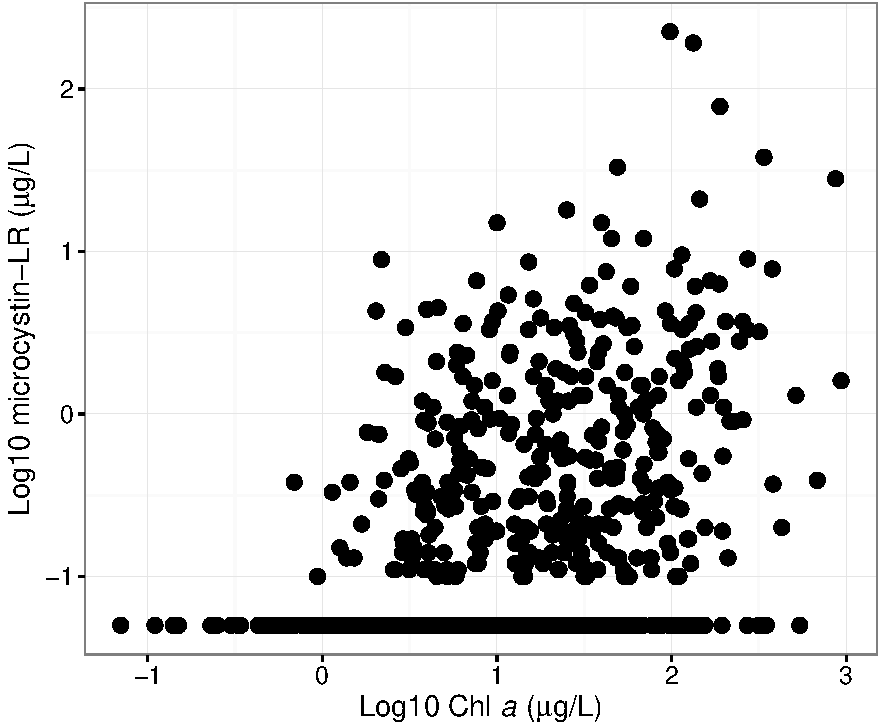
\includegraphics{manuscript_files/figure-latex/chla_micro_scatter-1.pdf}
\caption{Scatterplot showing association betweeen chlorophyll \textit{a}
and microcystin-LR. \label{fig:chla_micro_scatter}}
\end{figure}

\newpage

\begin{verbatim}
## Loading required package: grid
\end{verbatim}

\begin{figure}[htbp]
\centering
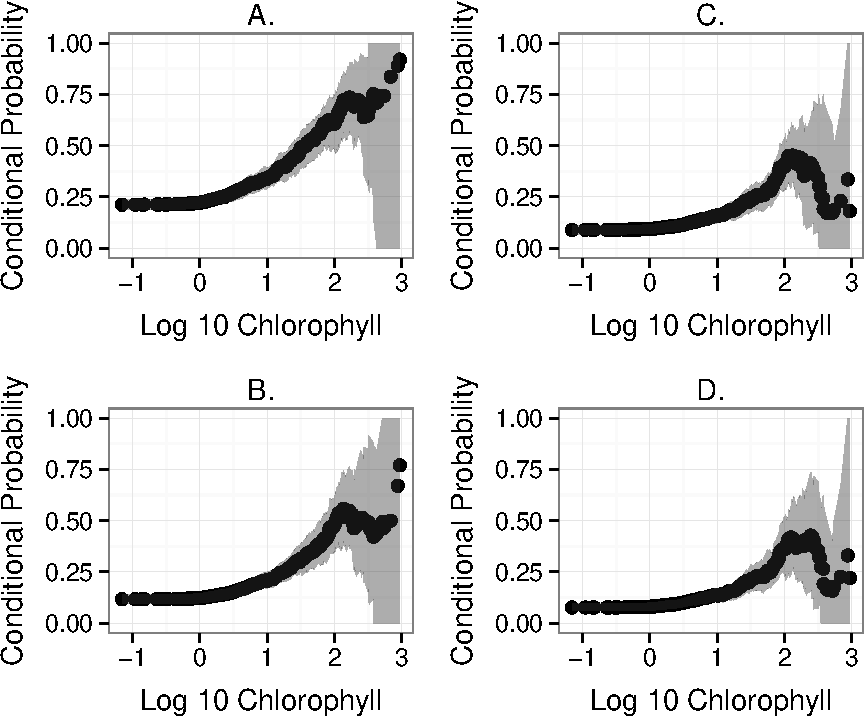
\includegraphics{manuscript_files/figure-latex/epa_child_cp_plot-1.pdf}
\caption{Conditional probability plots showing association between the
probability of exceeding various microcystin health advisory Levels. A.)
Plot for USEPA Child (0.3 \(\mu\)g/L). B.) Plot for WHO Drinking (1
\(\mu\)g/L). C.) Plot for USEPA Adult (1.6 \(\mu\)g/L). D.) Plot for WHO
Recreational (2 \(\mu\)g/L). \label{fig:multi_cp_plot}}
\end{figure}

\newpage

\section{Tables}\label{tables}

\begin{longtable}[c]{@{}lll@{}}
\caption{Various suggested microcystin health advisory concentrations.
\label{tab:microcystin_levels}}\tabularnewline
\toprule
Source & Type & Concentration\tabularnewline
\midrule
\endfirsthead
\toprule
Source & Type & Concentration\tabularnewline
\midrule
\endhead
USEPA & Child Drinking Water Advisory & 0.3 \(\mu\)g/L\tabularnewline
WHO & Drinking Water & 1 \(\mu\)g/L\tabularnewline
USEPA & Adult Drinking Water Advisory & 1.6 \(\mu\)g/L\tabularnewline
WHO & Recreational: Low Prob. of Effect & 2-4 \(\mu\)g/L\tabularnewline
WHO & Recreational: Moderate Prob. of Effect & 10-20
\(\mu\)g/L\tabularnewline
WHO & Recreational: High Prob. of Effect & 20-2000
\(\mu\)g/L\tabularnewline
WHO & Recreational: Very High Prob. of Effect & \textgreater{}2000
\(\mu\)g/L\tabularnewline
\bottomrule
\end{longtable}

\newpage

\begin{longtable}[c]{@{}lllll@{}}
\caption{Chlorophyll \textit{a} concentrations that are associated with
a 50\% probability of exceeding a microcystin health advisory
concentration. \label{tab:mc_chla_table}}\tabularnewline
\toprule
Cond. Probability U & SEPA Child (0.3 \(\mu\)g/L) W & HO Drink (1
\(\mu\)g/L) U & SEPA Adult (1.6 \(\mu\)g/L) W & HO Recreational (2
\(\mu\)g/L)\tabularnewline
\midrule
\endfirsthead
\toprule
Cond. Probability U & SEPA Child (0.3 \(\mu\)g/L) W & HO Drink (1
\(\mu\)g/L) U & SEPA Adult (1.6 \(\mu\)g/L) W & HO Recreational (2
\(\mu\)g/L)\tabularnewline
\midrule
\endhead
0.1 & 0.07 & 0.07 & 0.07 & 1\tabularnewline
0.2 & 0.07 & 5 & 11 & 15\tabularnewline
0.3 & 3 & 18 & 32 & 39\tabularnewline
0.4 & 11 & 39 & 67 & 78\tabularnewline
0.5 & 23 & 64 & 84 & 103\tabularnewline
0.6 & 39 & 92 & 115 & 167\tabularnewline
0.7 & 65 & 116 & 274 & 274\tabularnewline
0.8 & 115 & 256 & 871 & 871\tabularnewline
0.9 & 138 & 318 & 871 & 871\tabularnewline
\bottomrule
\end{longtable}

\newpage

\begin{longtable}[c]{@{}llll@{}}
\caption{Confusion matrix comparing chlorophyll \textit{a} predicted
exceedences (rows) versus real exceedances (columns) for the USEPA
childrens drinking water advisory.
\label{tab:child_conmat_table}}\tabularnewline
\toprule
Not Exceed Exc & eed Row Tot & als &\tabularnewline
\midrule
\endfirsthead
\toprule
Not Exceed Exc & eed Row Tot & als &\tabularnewline
\midrule
\endhead
Not Exceed & 344 & 78 & 422\tabularnewline
Exceed & 467 & 139 & 606\tabularnewline
Column Totals & 811 & 217 & 1028\tabularnewline
\bottomrule
\end{longtable}

\newpage

\begin{longtable}[c]{@{}llll@{}}
\caption{Confusion matrix comparing chlorophyll \textit{a} predicted
exceedences (rows) versus real exceedances (columns) for the WHO
drinking water advisory.
\label{tab:who_drink_conmat_table}}\tabularnewline
\toprule
Not Exceed Exc & eed Row Tot & als &\tabularnewline
\midrule
\endfirsthead
\toprule
Not Exceed Exc & eed Row Tot & als &\tabularnewline
\midrule
\endhead
Not Exceed & 787 & 98 & 885\tabularnewline
Exceed & 120 & 23 & 143\tabularnewline
Column Totals & 907 & 121 & 1028\tabularnewline
\bottomrule
\end{longtable}

\newpage

\begin{longtable}[c]{@{}llll@{}}
\caption{Confusion matrix comparing chlorophyll \textit{a} predicted
exceedences (rows) versus real exceedances (columns) for the USEPA adult
drinking water advisory. \label{tab:adult_conmat_table}}\tabularnewline
\toprule
Not Exceed Exc & eed Row Tot & als &\tabularnewline
\midrule
\endfirsthead
\toprule
Not Exceed Exc & eed Row Tot & als &\tabularnewline
\midrule
\endhead
Not Exceed & 897 & 82 & 979\tabularnewline
Exceed & 40 & 9 & 49\tabularnewline
Column Totals & 937 & 91 & 1028\tabularnewline
\bottomrule
\end{longtable}

\newpage

\begin{longtable}[c]{@{}llll@{}}
\caption{Confusion matrix comparing chlorophyll \textit{a} predicted
exceedences (rows) versus real exceedances (columns) for the WHO
recreational water advisory.
\label{tab:who_rec_conmat_table}}\tabularnewline
\toprule
Not Exceed Exc & eed Row Tot & als &\tabularnewline
\midrule
\endfirsthead
\toprule
Not Exceed Exc & eed Row Tot & als &\tabularnewline
\midrule
\endhead
Not Exceed & 61 & 2 & 63\tabularnewline
Exceed & 892 & 73 & 965\tabularnewline
Column Totals & 953 & 75 & 1028\tabularnewline
\bottomrule
\end{longtable}

\newpage

\section*{References}\label{references}
\addcontentsline{toc}{section}{References}

\hypertarget{refs}{}
\hypertarget{ref-jetoo2015toledo}{}
1. Jetoo S, Grover VI, Krantzberg G (2015) The toledo drinking water
advisory: Suggested application of the water safety planning approach.
Sustainability 7: 9787--9808.

\hypertarget{ref-rinta2009lake}{}
2. Rinta-Kanto JM, Konopko EA, DeBruyn JM, Bourbonniere RA, Boyer GL, et
al. (2009) Lake erie microcystis: Relationship between microcystin
production, dynamics of genotypes and environmental parameters in a
large lake. Harmful Algae 8: 665--673.

\hypertarget{ref-HABHRCA2014}{}
3. Bloom HA, Research H, Act CA (2014) Harmful Algal Bloom and Hypoxia
Research and Control Amendments Act of 2014. (S. 1254). Available:
\url{https://www.congress.gov/113/bills/s1254/BILLS-113s1254enr.pdf}.

\hypertarget{ref-mcelhiney2005detection}{}
4. McElhiney J, Lawton LA (2005) Detection of the cyanobacterial
hepatotoxins microcystins. Toxicology and Applied Pharmacology 203:
219--230.

\hypertarget{ref-zurawell2005hepatotoxic}{}
5. Zurawell RW, Chen H, Burke JM, Prepas EE (2005) Hepatotoxic
cyanobacteria: A review of the biological importance of microcystins in
freshwater environments. Journal of Toxicology and Environmental Health,
Part B 8: 1--37.

\hypertarget{ref-usepa2015drinking}{}
6. USEPA (2015) Drinking water health advisory for the cyanobacterial
microcystin toxins. EPA-820-R-15100. Available:
\url{http://www2.epa.gov/sites/production/files/2015-06/documents/microcystins-report-2015.pdf}.

\hypertarget{ref-world2003cyanobacterial}{}
7. World Health Organization (2003) Cyanobacterial toxins:
Microcystin-LR in drinking-water. Background document for development of
WHO guidelines for drinking-water quality. Geneva, Switzerland. World
Health Organization, 2nd ed. Geneva.

\hypertarget{ref-chorus1999toxic}{}
8. Chorus EI, Bartram J (1999) Toxic cyanobacteria in water: A guide to
their public health consequences, monitoring and management. World
Health Organization.

\hypertarget{ref-james2011environmental}{}
9. James R, Gregg A, Dindal A, McKernan J (2011) Environmental
technology verification report: Abraxis microcystin test kits. Online
document. Accessed online: June 22.

\hypertarget{ref-aranda2015evaluation}{}
10. Aranda-Rodriguez R, Jin Z, Harvie J, Cabecinha A (2015) Evaluation
of three field test kits to detect microcystins from a public health
perspective. Harmful Algae 42: 34--42.

\hypertarget{ref-yuan2015deriving}{}
11. Yuan LL, Pollard AI (2015) Deriving nutrient targets to prevent
excessive cyanobacterial densities in uS lakes and reservoirs.
Freshwater Biology 60: 1901--1916.

\hypertarget{ref-pip2014microcystin}{}
12. Pip E, Bowman L (2014) Microcystin and algal chlorophyll in relation
to nearshore nutrient concentrations in Lake Winnipeg, Canada.
Environment and Pollution 3: p36.

\hypertarget{ref-yuan2014managing}{}
13. Yuan LL, Pollard AI, Pather S, Oliver JL, D'Anglada L (2014)
Managing microcystin: Identifying national-scale thresholds for total
nitrogen and chlorophyll a. Freshwater Biology 59: 1970--1981.

\hypertarget{ref-usepa2009national}{}
14. USEPA (2009) National lakes assessment: A collaborative survey of
the nation's lakes. EPA 841-R-09-001.

\hypertarget{ref-nlaux5ffieldops}{}
15. USEPA (2007) Survey of the nation's lakes field operations manual
EPA841-B-07-004.

\hypertarget{ref-paul2011probability}{}
16. Paul JF, Munns WR (2011) Probability surveys, conditional
probability, and ecological risk assessment. Environmental Toxicology
and Chemistry 30: 1488--1495.

\hypertarget{ref-paul2005development}{}
17. Paul JF, McDonald ME (2005) Development of empirical, geographically
specific water quality criteria: A conditional probability analysis
approach. Journal of the American Water Resources Association 41:
1211--1223.

\hypertarget{ref-hollister2008cprob}{}
18. Hollister JW, Walker HA, Paul JF (2008) CProb: A computational tool
for conducting conditional probability analysis. Journal of
Environmental Quality 37: 2392--2396.

\hypertarget{ref-miller2013spatiotemporal}{}
19. Miller TR, Beversdorf L, Chaston SD, McMahon KD (2013)
Spatiotemporal molecular analysis of cyanobacteria blooms reveals
microcystis-aphanizomenon interactions. PloS one 8: e74933.

\hypertarget{ref-marion2012vivo}{}
20. Marion JW, Lee J, Wilkins III J, Lemeshow S, Lee C, et al. (2012) In
vivo phycocyanin flourometry as a potential rapid screening tool for
predicting elevated microcystin concentrations at eutrophic lakes.
Environmental science \& technology 46: 4523--4531.

\hypertarget{ref-beaver2014land}{}
21. Beaver JR, Manis EE, Loftin KA, Graham JL, Pollard AI, et al. (2014)
Land use patterns, ecoregion, and microcystin relationships in uS lakes
and reservoirs: A preliminary evaluation. Harmful Algae 36: 57--62.

\hypertarget{ref-wagner2011landscape}{}
22. Wagner T, Soranno PA, Webster KE, Cheruvelil KS (2011) Landscape
drivers of regional variation in the relationship between total
phosphorus and chlorophyll in lakes. Freshwater Biology 56: 1811--1824.

\end{document}